\documentclass[11pt,a4paper]{article}
\usepackage[margin=0.85in]{geometry}
\usepackage[T1]{fontenc}
\usepackage{lmodern,amsmath,amssymb,booktabs,array,tabularx,graphicx}
\usepackage[hidelinks]{hyperref}
\usepackage{caption,fancyhdr}
\captionsetup{font=small,labelfont=bf}
\pagestyle{fancy}\fancyhf{}
\fancyhead[L]{\small Supplementary methodological framework}
\fancyhead[R]{\small Revised supplement}
\fancyfoot[C]{\thepage}
\setlength{\headheight}{14pt}
\setlength{\parindent}{0pt}\setlength{\parskip}{5pt}
\setlength{\emergencystretch}{2em}
\renewcommand{\thesection}{S\arabic{section}}
\renewcommand{\thesubsection}{\thesection.\arabic{subsection}}
\renewcommand{\theequation}{S\arabic{equation}}
\renewcommand{\thetable}{S\arabic{table}}
\renewcommand{\thefigure}{S\arabic{figure}}
\newcommand{\family}[1]{\textbf{#1}}
\newcommand{\PoolCountSixteen}{260}
\newcommand{\PoolShareSixteen}{1.30\%}
\newcommand{\MinLossSixteen}{0.0104338}
\newcommand{\MLTIQRSixteen}{0.039}
\newcommand{\PoolCountTwentyOne}{3420}
\newcommand{\PoolShareTwentyOne}{17.10\%}
\newcommand{\MinLossTwentyOne}{0.0071058}
\newcommand{\MLTIQRTwentyOne}{0.095}

\begin{document}
\begin{center}
{\LARGE\bfseries Supplementary Material}\\[5pt]
{\large Inferring Institutionally Shaped Operational Constraints\\
in Power System Dispatch Models}\\[6pt]
Ziying Song, Yuanyuan Shi, and Michael R. Davidson
\end{center}
{\small\textit{Working revision:} S1--S5 use the final 100-run datasets and
the completed 2016 and 2021 original-UCED revalidation.}

\section{Forward UCED Formulation}
The forward model solves independent 168-hour weekly unit-commitment and
economic-dispatch (UCED) problems with fixed infrastructure. It co-optimizes
commitment, dispatch, zonal exchange, storage and reservoir operation, load
shedding, and upward/downward reserves. The formulation below groups the
implemented constraints and shows where the inferred parameters enter.
Notation follows HOPE where practical; the equations represent
\texttt{model/EDUCModel.jl}, not additional HOPE model options.

\begin{center}\small
\begin{tabularx}{\linewidth}{@{}lX@{}}\toprule
Symbol & Meaning \\\midrule
$h\in H,\ i\in I,\ l\in L$ & Hours, zones, and transmission corridors.\\
$G,G^{UC},G^{CHP},G^{VRE},G^{HY}$ & Generators; UC, CHP, wind/solar, and hydro subsets.\\
$s\in S,\ b\in B,\ A=G\cup S$ & Electrical storage, shedding segments, and all resources.\\
$p_{g,h},c_{s,h},dc_{s,h}$ & Generation, storage charging, and discharging (MW).\\
$o_{g,h},su_{g,h},sd_{g,h}$ & Binary online, startup, and shutdown indicators.\\
$soc_{a,h},q_{g,h}$ & Stored energy (MWh) and hydro spillage (MW equivalent).\\
$f^+_{l,h},f^-_{l,h},p^{LS}_{i,b,h}$ & Directional flows and unserved demand (MW).\\
$r^\uparrow_{a,h},r^\downarrow_{a,h},\xi^+_{l,h},\xi^-_{l,h}$ & Reserves and MLT-band relaxation slacks (MW).\\\bottomrule
\end{tabularx}
\end{center}
Subscripts $i$ on resource sets indicate location. Define $x_{a,h}=p_{a,h}$
for generators and $x_{a,h}=dc_{a,h}$ for storage. With one-hour steps,
the operating-cost objective is
\begin{align}
\min\quad &\sum_{h\in H}\omega_h\left[
\sum_{a\in A}VCG_{a,h}x_{a,h}+\sum_{i,b}VOLL_{i,b}p^{LS}_{i,b,h}\right]
\nonumber\\
&+\sum_{g\in G^{UC},h}STC_{g,h}P_g^{unit}su_{g,h}
+\pi^{MLT}\sum_{l,h}(\xi^+_{l,h}+\xi^-_{l,h}).\label{eq:objective}
\end{align}
$VCG$, $VOLL$, and $STC P^{unit}$ denote dispatch, shedding, and startup
costs; $P^{unit}$ is the input unit size. The current weights are
$\omega_h=1$, and $\pi^{MLT}=10^7$. Capacity auxiliaries in the code are
fixed to existing capacities and written here as parameters.

\family{Power balance and shedding.} For every zone/hour,
\begin{equation}
\sum_{g\in G_i}p_{g,h}+\sum_{s\in S_i}(dc_{s,h}-c_{s,h})
+\sum_l\Phi_{i,l,h}+\sum_b p^{LS}_{i,b,h}=Load_{i,h},
\quad 0\le\sum_b p^{LS}_{i,b,h}\le Load_{i,h}.\label{eq:balance}
\end{equation}
$\Phi$ is loss-adjusted net corridor injection. All continuous operating
variables are nonnegative. The remaining constraint families follow.

\newpage
\family{Output, commitment, and ramping.}
\begin{align}
AF_{g,h}\chi_{g,w}\mu_gP_g^{max}o_{g,h}
&\le p_{g,h}\le AF_{g,h}P_g^{max}o_{g,h},&&g\in G^{UC},\label{eq:output}\\
\mu_aP_a^{max}\le x_{a,h}&\le AF_{a,h}P_a^{max},&&a\in A\setminus G^{UC},\\
(\boldsymbol{o}_g,\boldsymbol{su}_g,\boldsymbol{sd}_g,\boldsymbol{p}_g)
&\in\mathcal U_g(\mu_g,P_g^{max},RU_g,RD_g,UT_g,DT_g),&&g\in G^{UC}.
\end{align}
$AF$ is hourly availability and $\mu$ the minimum-output fraction.
$\mathcal U_g$ collects status transitions, binary bounds, minimum up/down
windows, and commitment-adjusted ramp limits. Non-UC resources have ordinary
up/down ramp limits. Wind/solar curtailment equals available output minus
dispatch. Non-UC minimum output is zero in the intended inputs.

\family{Seasonal CHP.} During heating weeks,
\begin{equation}
\sum_{g\in G^{CHP}}P_g^{max}o_{g,h}\ge
0.80\sum_{g\in G^{CHP}}P_g^{max}.\label{eq:chp}
\end{equation}
For CHP, $\chi_{g,w}$ is 1.20 in deep winter, 1.05 in shoulder heating weeks,
and 1 otherwise; for non-CHP units it is always 1. Heating weeks are 1--15
and 42--52; deep-winter weeks are 1--8 and 46--52.

\family{Storage and reservoir hydro.} At hourly resolution,
\begin{align}
soc_{s,h}&=soc_{s,h-1}+\eta_s^{ch}c_{s,h}-dc_{s,h}/\eta_s^{dis},
&0\le soc_{s,h}\le E_s^{max},\\
soc_{g,h}&=soc_{g,h-1}+I_{g,h}-q_{g,h}-p_{g,h}/\eta_g^{dis},
&\beta E_g^{max}\le soc_{g,h}\le E_g^{max}.
\end{align}
The first row applies to $s\in S$ and the second to $g\in G^{HY}$.
Hydro inflow is $I_{g,h}=AF_{g,h}P_g^{max}\eta_g^{ch}$, with
$0\le q_{g,h}\le I_{g,h}$. Initial energy is $\alpha E^{max}$; final storage
energy may differ by $\pm0.1E^{max}$, while hydro returns to its initial level.
Storage has a shared charging/discharging/reserve power limit. There is no
binary charging/discharging exclusivity. $\alpha$ and $\beta$ are input fractions.

\family{Transmission and MLT schedules.} Set $\kappa_l=1-\ell_l/2$ for loss
fraction $\ell_l$. Directional flows satisfy $0\le f^\pm_{l,h}\le\kappa_lF_l^{max}$.
The code uses $\Phi_{i,l,h}=-\sum_{d\in\{+,-\}}[A^d_{i,l}f^d_{l,h}
+|A^d_{i,l}|\ell_l f^d_{l,h}/(2\kappa_l)]$, with incidence $+1$ at the sender
and $-1$ at the receiver. For signed delivery benchmark $m_{l,h}$,
\begin{equation}
(1-\delta)|m_{l,h}|\kappa_l-\xi^-_{l,h}\le f^{dir}_{l,h}
\le(1+\delta)|m_{l,h}|\kappa_l+\xi^+_{l,h},\quad f^{opp}_{l,h}=0.\label{eq:mlt}
\end{equation}
The direction follows the benchmark sign. These schedule restrictions apply
in PriorityMLT; SpotOnly omits them. Physical limits and designated one-way
external exports remain. MLT slacks provide a numerical/modeling relaxation
and diagnostic; they do not define an inference admissibility classifier.

\family{Zonal reserves.} Resource-specific sets $\mathcal R_a$ collect power
headroom, ramping, and storage/hydro energy limits. For every zone/hour,
\begin{align}
(r^\uparrow_{a,h},r^\downarrow_{a,h})&\in\mathcal R_a(x,o,c,soc),\nonumber\\
\sum_{a\in A_i}r^\uparrow_{a,h}&\ge\lambda_i^DLoad_{i,h}
+\lambda_i^{VRE}\sum_{g\in G_i\cap G^{VRE}}p_{g,h}+Q_i,\\
\sum_{a\in A_i}r^\downarrow_{a,h}&\ge\lambda_i^DLoad_{i,h}
+\lambda_i^{VRE}\sum_{g\in G_i\cap G^{VRE}}p_{g,h}.
\end{align}
$Q_i$ is the configured largest-unit/interconnection contingency. The
inferred vector $\theta=(\delta,\{\mu_k,\tau_k\}_k)$ enters the MLT band,
minimum-output bounds, and UC windows ($UT_g=DT_g=\mathrm{round}(\tau_k)$
for units in class $k$). Other inputs remain fixed within each year's inference.

\newpage
\section{Candidate Parameterization and Preliminary Screening}
\subsection{Preliminary coal-side screening}
The preliminary exercise described in the original supplement compared CHP
and non-CHP coal parameter responses over a three-month design. CHP
minimum-output parameters showed the clearer coal-generation response,
especially in the two smaller size classes. Non-CHP parameters showed limited
response under that design and were not carried into the full-year inference
experiment. This is a design-specific screening result, not a claim that
non-CHP flexibility is generally unimportant or intrinsically unrecoverable.
No new preliminary-screening estimates are introduced in this revision.

\subsection{Candidate domain and generator grouping}
The initial experiment uses a 100-point LHS design over a prespecified
13-dimensional domain: six minimum-output fractions, six common minimum
up/down-time controls, and one MLT band. Table~\ref{tab:domain} lists the
fixed domain boundaries, not realized sample minima and maxima.

\textbf{R} denotes official retrofitted coal pilot units, including both CHP
and conventional coal where present. \textbf{C} denotes non-retrofitted CHP.
These groups are crossed with three capacity classes in MW. The time control
is sampled numerically and rounded to an integer before being assigned to
both minimum up and down times. Other non-retrofitted conventional coal
units use fixed minimum output 0.40 and up/down-time inputs of 8 hours in
the current input-generation workflow.

\begin{center}
\captionof{table}{Complete candidate domain. ``min'' is a capacity fraction;
``time'' is in hours. All 13 dimensions belong to the initial design in both years.}
\label{tab:domain}
\small\begin{tabular}{@{}llrrl@{}}
\toprule
ID & Parameter & 2016 bounds & 2021 bounds & Years \\
\midrule
P1 & R-min 660-1000 & [0.30, 0.75] & [0.30, 0.75] & Both \\
P2 & R-time 660-1000 & [4.00, 16.00] & [4.00, 8.00] & Both \\
P3 & R-min 300-660 & [0.30, 0.75] & [0.30, 0.75] & Both \\
P4 & R-time 300-660 & [4.00, 16.00] & [4.00, 8.00] & Both \\
P5 & R-min 0-300 & [0.30, 0.75] & [0.30, 0.75] & Both \\
P6 & R-time 0-300 & [4.00, 12.00] & [2.00, 6.00] & Both \\
P7 & C-min 660-1000 & [0.30, 0.75] & [0.30, 0.75] & Both \\
P8 & C-time 660-1000 & [4.00, 16.00] & [4.00, 16.00] & Both \\
P9 & C-min 300-660 & [0.30, 0.75] & [0.30, 0.75] & Both \\
P10 & C-time 300-660 & [4.00, 16.00] & [4.00, 16.00] & Both \\
P11 & C-min 0-300 & [0.30, 0.75] & [0.30, 0.75] & Both \\
P12 & C-time 0-300 & [4.00, 12.00] & [4.00, 12.00] & Both \\
P13 & MLT band & [0.05, 0.40] & [0.05, 0.40] & Both \\
\bottomrule
\end{tabular}

\end{center}

Retrofitted coal is a policy-defined group, whereas CHP and its seasonal
constraints are technology-defined. Legacy exploration files use
\texttt{CHP\_Retrofitted\_*} as an alias for
\texttt{Coal\_Retrofitted\_*}; the alias does not imply that all retrofitted
units are CHP. Only the technology-defined CHP subset receives the seasonal
multiplier in S1.

Year-specific time bounds are taken from the frozen
\texttt{lhs\_design\_domain.json} files. Their metadata documents reconstruction
of the original LHS bounds from stratification, rather than use of realized
extrema as new limits. The 2021 retrofitted-unit time bounds differ from 2016;
they should not be replaced by the current shared configuration when
reproducing the archived experiments.

The 100 evaluations in each year are partitioned into 80 development observations
and 20 independent held-out observations. The held-out observations are excluded
from GP fitting, cross-validation, and ARD screening.

\newpage
\section{GP Training, Validation, and ARD Screening}
\subsection{Specification and validation}
The response is the same quantity mismatch as in the main paper:
\begin{equation}
L(\theta)=\tfrac14\left(E_{coal}^2+E_{wind}^2+E_{solar}^2+E_{exchange}^2\right).
\end{equation}
Generation errors use capacity-normalized regional RMSE, averaged with equal
regional weights; exchange uses the observed-flow normalization described
in the main paper. No square root is taken after the weighted squared
component sum. The saved transformations for both years apply no Box--Cox
transformation. Inputs and loss are centered and scaled using training data,
with fold-specific preprocessing during cross-validation.

The reported models use zero-mean GPs with ARD Mat\'ern kernels. The final
2016 fit uses Mat\'ern $5/2$, while the final 2021 fit uses Mat\'ern $3/2$:
\begin{equation}
\begin{aligned}
k_{3/2}(z,z')&=\sigma_f^2(1+\sqrt3r)\exp(-\sqrt3r),\\
k_{5/2}(z,z')&=\sigma_f^2(1+\sqrt5r+5r^2/3)\exp(-\sqrt5r),\\
r^2&=\sum_j(z_j-z'_j)^2/\ell_j^2.
\end{aligned}
\end{equation}
A single fitted nugget $\sigma_n^2$ enters the covariance diagonal.
It accommodates numerical tolerances and unresolved response variation;
it is not an estimated uncertainty distribution over institutional parameters.
The kernel family is held fixed in the reported ARD and reduced-GP fits.
The saved-model evidence does not require retaining the old supplement's
nested kernel-selection or composite NLL/coverage selection procedure.

\begin{center}
\captionof{table}{GP configuration used for the reported fits. Bounds are in natural logs.}
\small
\begin{tabularx}{\linewidth}{@{}lX@{}}\toprule
Item & Setting \\\midrule
Kernel and mean & Mat\'ern $5/2$ ARD (2016) and Mat\'ern $3/2$ ARD (2021); zero mean after standardization.\\
Hyperparameter estimation & Bounded maximum marginal likelihood; no hyperpriors.\\
Bounds & $\log\ell_j\in[-3,4]$; $\log\sigma_f\in[-3,3]$;
$\log\sigma_n\in[\log(10^{-3}),\log(0.5)]$.\\
Three initializations & $\ell_j\in\{0.5,1,2\}$, with $\sigma_f=1$, $\sigma_n=0.05$.\\
Validation & Saved independent test partition; five development folds.\\
ARD criterion & Drop when $\log\ell_j\ge3.9$ in at least four of five fits.\\\bottomrule
\end{tabularx}
\end{center}

\begin{center}
\captionof{table}{Latest full- and reduced-GP validation. Test predictions were
regenerated from each saved model on its frozen held-out rows.}
\label{tab:performance}
\small\begin{tabular}{@{}llrrrrr@{}}
\toprule
Year & GP & CV $R^2$ & CV RMSE$^{a}$ & Test $R^2$ & Test RMSE$^{b}$ & $n_{test}$ \\
\midrule
2016 & Full & 0.9982 & 0.0424 & 0.9979 & 1.387 & 20 \\
2016 & Reduced & 0.9988 & 0.0343 & 0.9987 & 1.084 & 20 \\
2021 & Full & 0.9790 & 0.1440 & 0.9936 & 1.389 & 20 \\
2021 & Reduced & 0.9853 & 0.1204 & 0.9933 & 1.419 & 20 \\
\bottomrule
\end{tabular}

\end{center}
{\footnotesize $^a$CV RMSE uses the saved standardized responses; pooled CV
$R^2$ is reported, not the mean of fold $R^2$ values.
$^b$Test RMSE is on the original loss scale, in units of $10^{-4}$.
Both current test sets contain 20 observations.}

The held-out data serve reporting rather than kernel or feature selection.
Test $R^2$ uses the held-out mean as the constant reference. The reduced models
achieve test $R^2=0.9987$ in 2016 and 0.9933 in 2021, with original-scale
RMSE of $1.08\times10^{-4}$ and $1.42\times10^{-4}$, respectively. Relative
to the corresponding full fits, the reduced fit improves the 2016 test metrics
slightly and changes the 2021 metrics only marginally: test $R^2$ changes from
0.9936 to 0.9933 and RMSE from $1.39\times10^{-4}$ to $1.42\times10^{-4}$.
Saved reduced-GP 95\% predictive-interval coverage is 90\% for 2016 and
100\% for 2021.

\newpage
\subsection{Fold-wise ARD screening criterion}
Let $\widehat\ell_j^{(f)}$ be the length scale estimated using the training
portion of development fold $f$. The fixed criterion is
\begin{equation}
v_j=\sum_{f=1}^{5}\mathbf1\{\log\widehat\ell_j^{(f)}\ge4-0.1\},
\qquad j\text{ is screened out if }v_j\ge4.
\end{equation}
The complete results are shown below. An upper-bound length scale indicates
weak resolved variation of the loss along a dimension over the sampled domain.
ARD does not establish parameter recoverability; that question requires the
low-mismatch-region diagnostics in S4.

\begin{center}
\captionof{table}{Full 13-dimensional ARD screening. F1--F5 are fitted log length
scales; hits are counted before rounding. R/C labels follow Table~\ref{tab:domain}.}
\label{tab:ard}
\fontsize{8.5}{10.3}\selectfont
\setlength{\tabcolsep}{4pt}\renewcommand{\arraystretch}{1.10}
\begin{tabular}{@{}llrrrrrrl@{}}
\toprule
Year & Parameter & F1 & F2 & F3 & F4 & F5 & Hits & Rule \\
\midrule
2016 & R-min 660-1000 & 4.00 & 4.00 & 4.00 & 4.00 & 4.00 & 5/5 & Drop \\
2016 & R-time 660-1000 & 4.00 & 4.00 & 4.00 & 4.00 & 4.00 & 5/5 & Drop \\
2016 & R-min 300-660 & 4.00 & 4.00 & 4.00 & 4.00 & 4.00 & 5/5 & Drop \\
2016 & R-time 300-660 & 4.00 & 4.00 & 4.00 & 4.00 & 4.00 & 5/5 & Drop \\
2016 & R-min 0-300 & 4.00 & 4.00 & 4.00 & 4.00 & 4.00 & 5/5 & Drop \\
2016 & R-time 0-300 & 4.00 & 4.00 & 4.00 & 4.00 & 4.00 & 5/5 & Drop \\
2016 & C-min 660-1000 & 4.00 & 4.00 & 4.00 & 4.00 & 4.00 & 5/5 & Drop \\
2016 & C-time 660-1000 & 4.00 & 4.00 & 4.00 & 4.00 & 4.00 & 5/5 & Drop \\
2016 & C-min 300-660 & 2.18 & 2.06 & 2.00 & 2.07 & 2.06 & 0/5 & Retain \\
2016 & C-time 300-660 & 4.00 & 4.00 & 4.00 & 3.85 & 4.00 & 4/5 & Drop \\
2016 & C-min 0-300 & 2.07 & 2.11 & 1.99 & 2.06 & 2.17 & 0/5 & Retain \\
2016 & C-time 0-300 & 4.00 & 4.00 & 4.00 & 4.00 & 4.00 & 5/5 & Drop \\
2016 & MLT band & 1.29 & 1.40 & 1.26 & 1.31 & 1.23 & 0/5 & Retain \\
2021 & R-min 660-1000 & 4.00 & 4.00 & 4.00 & 3.41 & 4.00 & 4/5 & Drop \\
2021 & R-time 660-1000 & 4.00 & 4.00 & 4.00 & 4.00 & 4.00 & 5/5 & Drop \\
2021 & R-min 300-660 & 2.52 & 2.67 & 2.49 & 2.37 & 2.39 & 0/5 & Retain \\
2021 & R-time 300-660 & 4.00 & 4.00 & 4.00 & 4.00 & 4.00 & 5/5 & Drop \\
2021 & R-min 0-300 & 2.73 & 4.00 & 2.74 & 4.00 & 4.00 & 3/5 & Retain \\
2021 & R-time 0-300 & 4.00 & 3.13 & 2.86 & 4.00 & 3.02 & 2/5 & Retain \\
2021 & C-min 660-1000 & 4.00 & 4.00 & 4.00 & 3.92 & 4.00 & 5/5 & Drop \\
2021 & C-time 660-1000 & 4.00 & 4.00 & 4.00 & 4.00 & 4.00 & 5/5 & Drop \\
2021 & C-min 300-660 & 2.03 & 2.51 & 2.49 & 1.65 & 2.14 & 0/5 & Retain \\
2021 & C-time 300-660 & 4.00 & 4.00 & 3.62 & 4.00 & 4.00 & 4/5 & Drop \\
2021 & C-min 0-300 & 2.34 & 2.49 & 2.50 & 2.45 & 2.51 & 0/5 & Retain \\
2021 & C-time 0-300 & 4.00 & 4.00 & 4.00 & 4.00 & 4.00 & 5/5 & Drop \\
2021 & MLT band & 0.84 & 1.06 & 0.99 & 1.09 & 1.16 & 0/5 & Retain \\
\bottomrule
\end{tabular}

\end{center}

\subsection{Reduced GP and retained dimensions}
The 2016 baseline screening retains three parameters: MLT band and
non-retrofitted CHP minimum output in the 300--660 and 0--300 MW groups.
The 2021 baseline retains these three plus retrofitted-coal minimum output
in the 300--660 and 0--300 MW groups and retrofitted-coal minimum up/down
time in the 0--300 MW group, for six retained dimensions in total.

The reduced GP is refitted using only these retained coordinates from the
development design. It approximates the reduced empirical response represented
by that design. It is neither the loss conditional on a particular value of
the discarded parameters nor an exact analytical marginalization over them.
Variation in omitted dimensions can contribute to residual variation.

The 2021 R-min 0--300 dimension reaches the ceiling in three folds and the
R-time 0--300 dimension in two folds. Both therefore remain below the specified
four-of-five exclusion threshold. A rounded median log length scale alone would
not reproduce these fold-wise decisions.

\newpage
\subsection*{Screening stability and cross-fitted validation}
The upper-bound check repeats five-fold screening with \emph{length-scale}
ceilings multiplied by $0.5$, 1, and 2: log ceilings $4+\log(0.5)$, 4, and
$4+\log2$. The hit tolerance remains 0.1 log units.
\begin{center}
\captionof{table}{Ceiling hits under alternative upper bounds. Four or more hits
imply exclusion under that setting.}
\small\setlength{\tabcolsep}{4pt}\begin{tabular}{@{}lrrrrrr@{}}
\toprule
Parameter & 2016: $0.5\times$ & $1\times$ & $2\times$ & 2021: $0.5\times$ & $1\times$ & $2\times$ \\
\midrule
R-min 660-1000 & 5/5 & 5/5 & 5/5 & 5/5 & 4/5 & 4/5 \\
R-time 660-1000 & 5/5 & 5/5 & 5/5 & 5/5 & 5/5 & 5/5 \\
R-min 300-660 & 5/5 & 5/5 & 5/5 & 0/5 & 0/5 & 0/5 \\
R-time 300-660 & 5/5 & 5/5 & 5/5 & 5/5 & 5/5 & 5/5 \\
R-min 0-300 & 5/5 & 5/5 & 5/5 & 3/5 & 3/5 & 3/5 \\
R-time 0-300 & 5/5 & 5/5 & 5/5 & 3/5 & 2/5 & 2/5 \\
C-min 660-1000 & 5/5 & 5/5 & 5/5 & 5/5 & 5/5 & 4/5 \\
C-time 660-1000 & 5/5 & 5/5 & 3/5 & 5/5 & 5/5 & 5/5 \\
C-min 300-660 & 0/5 & 0/5 & 0/5 & 0/5 & 0/5 & 0/5 \\
C-time 300-660 & 5/5 & 4/5 & 5/5 & 5/5 & 4/5 & 4/5 \\
C-min 0-300 & 0/5 & 0/5 & 0/5 & 0/5 & 0/5 & 0/5 \\
C-time 0-300 & 5/5 & 5/5 & 5/5 & 5/5 & 5/5 & 4/5 \\
MLT band & 0/5 & 0/5 & 0/5 & 0/5 & 0/5 & 0/5 \\
\bottomrule
\end{tabular}

\end{center}
The 2021 retain/drop set is unchanged across the three tested ceilings.
In 2016, doubling the ceiling changes C-time 660--1000 from excluded
to retained: its ceiling-hit count falls from five to three. The three
parameters retained by the 2016 baseline remain retained under every tested
ceiling, but the complete 2016 retain/drop set is therefore not invariant
to the upper-bound specification.

A five-outer-fold check repeats five-fold ARD inside each outer training set
and compares full/reduced predictions on the excluded fold, addressing
selection leakage in fixed-active-set CV.
\begin{center}
\captionof{table}{Cross-fitted full/reduced comparison. RMSE is in standardized
response units; the change is relative to the full model.}
\small\begin{tabular}{@{}lrrrrr@{}}
\toprule
Year & Full $R^2$ & Reduced $R^2$ & Full RMSE & Reduced RMSE & $\Delta$ RMSE \\
\midrule
2016 & 0.9981 & 0.9988 & 0.0433 & 0.0343 & -20.74\% \\
2021 & 0.9790 & 0.9824 & 0.1440 & 0.1321 & -8.26\% \\
\bottomrule
\end{tabular}

\end{center}
The cross-fitted reduced models improve aggregate out-of-fold prediction:
RMSE decreases by 20.74\% in 2016 and 8.26\% in 2021. The corresponding
$R^2$ values change from 0.9981 to 0.9988 and from 0.9790 to 0.9824.
The archived overall robustness status is FAIL\_REVIEW for 2016 because
of its ceiling sensitivity and PASS for 2021.

\begin{center}
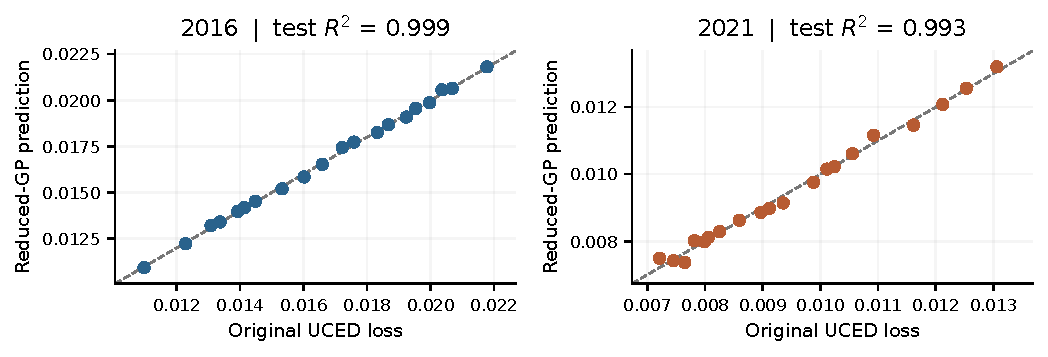
\includegraphics[width=.90\linewidth]{figures/holdout_validation.pdf}
\captionof{figure}{Latest reduced-GP predictions on independent held-out
evaluations. Dashed lines indicate equality; no points are removed from the plots.}
\end{center}

\newpage
\section{Low-Mismatch Region and Recoverability Diagnostics}
\subsection{Definition and primary region}
For each year, the latest saved reduced GP is evaluated on the same stored
20,000-point stratified LHS pool in retained-parameter space (seed 123).
The coordinates span the domain in S2; no original UCED solves are added.
With $\widehat L_{min}$ denoting the minimum predicted loss in that pool,
\begin{equation}
S_\epsilon=\{\theta_A\text{ in the evaluated pool}:\widehat L(\theta_A)
\le(1+\epsilon)\widehat L_{min}\},\qquad \epsilon=0.10.
\end{equation}
This finite-pool approximation describes a relative low-mismatch region,
not a confidence or credible region. Its reference minimum is not asserted
to be a global optimum. For dimension $j$, concentration is summarized by
\begin{equation}
\mathrm{nIQR}_j(S_\epsilon)=
\frac{Q_{0.75}(\theta_j\mid S_\epsilon)-Q_{0.25}(\theta_j\mid S_\epsilon)}{U_j-L_j}.
\end{equation}
$[L_j,U_j]$ is the corresponding design domain. Lower nIQR indicates greater
concentration within this pool and tolerance, not unique identification.

The refreshed pool minima are \MinLossSixteen{} in 2016 and
\MinLossTwentyOne{} in 2021. The primary regions contain
\PoolCountSixteen{} (\PoolShareSixteen{}) and
\PoolCountTwentyOne{} (\PoolShareTwentyOne{}) of their respective pools.
Both stored pools were evaluated with their final saved reduced GP models for
a consistent reporting snapshot.

\begin{center}
\captionof{table}{Retained-parameter distributions within the latest $S_{10\%}$.
All listed parameters are dimensionless. Min/max are finite-pool extrema.}
\label{tab:region}
\fontsize{9}{11}\selectfont\setlength{\tabcolsep}{4pt}
\begin{tabular}{@{}llrrrrrr@{}}
\toprule
Year & Parameter & Min & Q25 & Median & Q75 & Max & nIQR \\
\midrule
2016 & C-min 300-660 & 0.501 & 0.633 & 0.677 & 0.719 & 0.749 & 0.192 \\
2016 & C-min 0-300 & 0.477 & 0.621 & 0.669 & 0.714 & 0.748 & 0.208 \\
2016 & MLT band & 0.050 & 0.054 & 0.060 & 0.068 & 0.095 & 0.039 \\
2021 & R-min 300-660 & 0.300 & 0.446 & 0.559 & 0.659 & 0.750 & 0.473 \\
2021 & R-min 0-300 & 0.300 & 0.422 & 0.536 & 0.645 & 0.750 & 0.495 \\
2021 & R-time 0-300 & 2.001 & 3.177 & 4.198 & 5.112 & 5.997 & 0.484 \\
2021 & C-min 300-660 & 0.301 & 0.436 & 0.528 & 0.648 & 0.750 & 0.473 \\
2021 & C-min 0-300 & 0.300 & 0.416 & 0.530 & 0.639 & 0.750 & 0.495 \\
2021 & MLT band & 0.050 & 0.065 & 0.080 & 0.098 & 0.167 & 0.095 \\
\bottomrule
\end{tabular}

\end{center}

\begin{center}
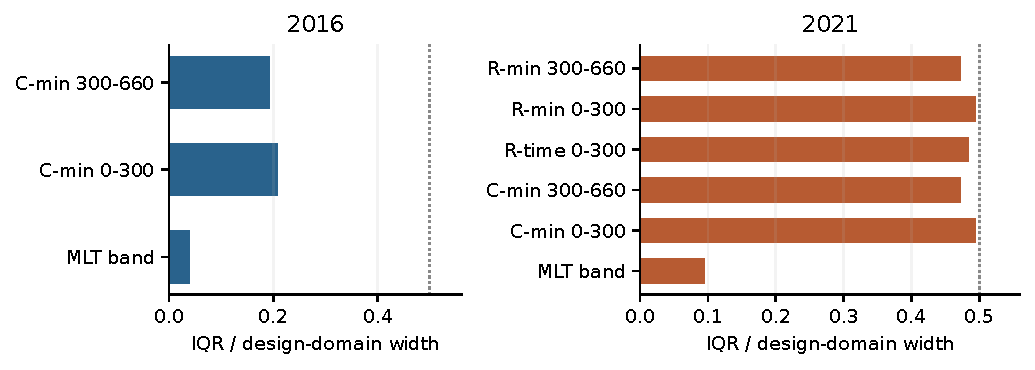
\includegraphics[width=.96\linewidth]{figures/normalized_iqr.pdf}
\captionof{figure}{Domain-normalized dispersion in $S_{10\%}$. The dotted
0.5 reference is the IQR of a uniform distribution over the full domain,
not a statistical decision threshold.}
\end{center}
MLT is more concentrated than the retained coal minimum-output parameters
in both years (nIQR \MLTIQRSixteen{} and \MLTIQRTwentyOne{}).
The additional 2021 retrofitted-coal dimensions have nIQR near 0.5:
their ARD relevance does not translate into narrow parameter-level ranges.

\newpage
\subsection{Tolerance sensitivity and joint relationships}
\begin{center}
\captionof{table}{Normalized IQR under alternative relative mismatch tolerances.}
\small\begin{tabular}{@{}llrrrr@{}}
\toprule
Year & Parameter & $5\%$ & $10\%$ & $20\%$ & $30\%$ \\
\midrule
2016 & C-min 300-660 & 0.121 & 0.192 & 0.395 & 0.472 \\
2016 & C-min 0-300 & 0.123 & 0.208 & 0.378 & 0.472 \\
2016 & MLT band & 0.020 & 0.039 & 0.065 & 0.094 \\
2021 & R-min 300-660 & 0.330 & 0.473 & 0.491 & 0.497 \\
2021 & R-min 0-300 & 0.495 & 0.495 & 0.501 & 0.501 \\
2021 & R-time 0-300 & 0.476 & 0.484 & 0.497 & 0.499 \\
2021 & C-min 300-660 & 0.442 & 0.473 & 0.488 & 0.486 \\
2021 & C-min 0-300 & 0.474 & 0.495 & 0.503 & 0.500 \\
2021 & MLT band & 0.047 & 0.095 & 0.177 & 0.242 \\
\bottomrule
\end{tabular}

\end{center}
\begin{center}
\captionof{table}{Number of pool members in each tolerance region; each pool
contains 20,000 points.}
\small\begin{tabular}{@{}lrrrr@{}}
\toprule
Year & $5\%$ & $10\%$ & $20\%$ & $30\%$ \\
\midrule
2016 & 53 & 260 & 1569 & 3415 \\
2021 & 859 & 3420 & 7041 & 9676 \\
\bottomrule
\end{tabular}

\end{center}
The MLT band remains the most concentrated retained dimension at each tested
tolerance in both years. Its range broadens as the tolerance increases,
especially in 2021. Coal-parameter dispersion is also tolerance-dependent;
the narrowest 2016 region has relatively few sampled members and should not
be read as a precise interval estimate. All summaries remain conditional on
the parameter bounds and the fitted reduced surface.

\begin{center}
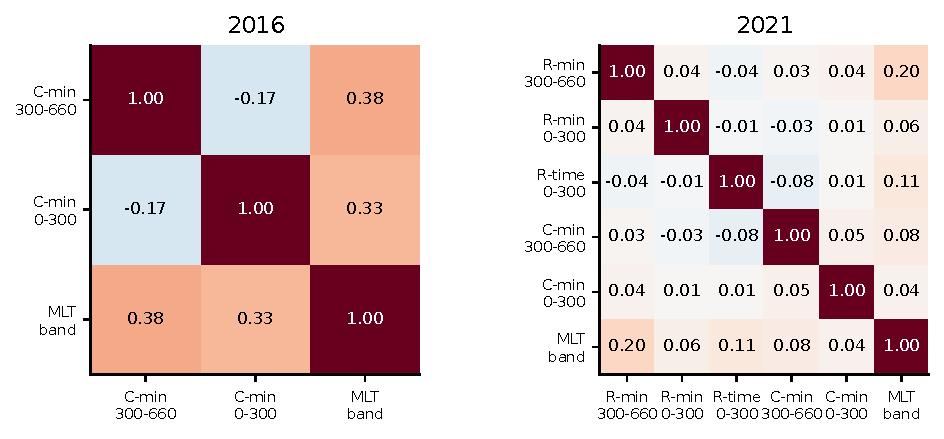
\includegraphics[width=.97\linewidth]{figures/pairwise_geometry.pdf}
\captionof{figure}{Spearman rank correlations among retained parameters within
the latest $S_{10\%}$. These describe the selected region's geometry;
they are neither causal effects nor tests of structural identification.}
\end{center}
The 2016 region exhibits a clearer negative relationship between the two
non-retrofitted CHP minimum-output dimensions than the corresponding 2021
region. Relationships with MLT can reflect compensation between delivery
flexibility and minimum-generation rigidity, but pairwise association alone
does not establish a unique mechanism. The weak 2021 coal--coal correlations
also illustrate that broad parameter ranges need not follow a single narrow
tradeoff curve.

\newpage
\subsection*{Interpretation and scope of the region diagnostics}
\begin{center}
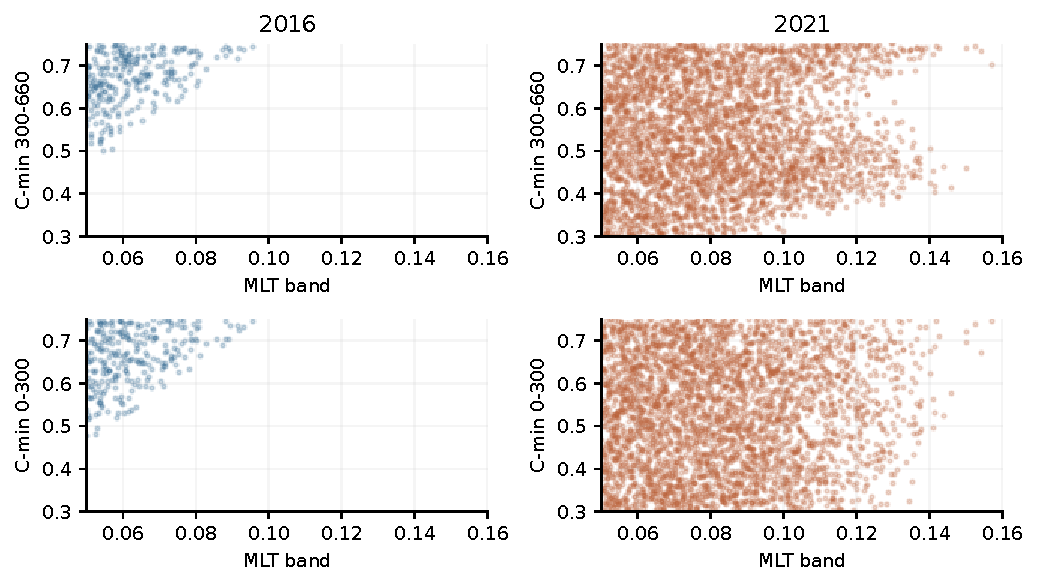
\includegraphics[width=.84\linewidth]{figures/joint_region.pdf}
\captionof{figure}{Pairwise projections of $S_{10\%}$ for MLT and the two
shared non-retrofitted CHP minimum-output parameters. All region members
are plotted; the MLT axis spans the full ex-ante domain $[0.05,0.40]$.
Projections conceal variation in other retained dimensions.}
\end{center}
The evidence supports different levels of interpretation across parameters.
MLT has a relatively concentrated model-ready delivery representation;
the coal minimum-output dimensions support a broader diagnosis of operating
rigidity. None of these sets uniquely identifies a policy or a causal reform
effect. Cross-year differences are interpreted as regime-specific effective
UCED representations, conditional on each year's inputs, observations, and
parameter domain.

The lower MLT domain boundary is 0.05. Concentration near this edge cannot
show whether a still narrower band would also match the quantities, because
that region was not evaluated. The 2016 screening sensitivity in S3 and the
limited spatial coverage of
the six-point-per-year revalidation in S5 constrain how specifically the surrogate
region can be interpreted. In particular, GP--UCED residuals at
fixed values of omitted parameters can combine approximation error and
variation associated with those parameters; they are not a formal upper bound
on either component.

\newpage
\section{Original-UCED Revalidation and Quantity Matching}
For each year, six parameter vectors were evaluated using the original UCED:
a center representative (labeled ``medoid'' in the files), four interior
points, and a surrogate-best point. Roles refer to the respective archived
selection, not a new optimization. GP predictions below use each year's
current reduced model at the exact evaluated coordinates; this accounts for
rounding continuous candidate parameters to three decimals before UCED runs.
All twelve parameter vectors match their archived candidate records.

\subsection{2016 revalidation}
The center representative is nearest the region centroid in domain-normalized
coordinates, and the four interior points span distance quartiles within the
region. The surrogate-best point is the lowest-predicted-loss pool member.
All six satisfy the final 2016 $S_{10\%}$ cutoff, approximately 0.011477.
Omitted parameters remain fixed at their prescribed midpoint values.

\begin{center}
\captionof{table}{2016 original-UCED revalidation. Losses are on the original
scale; residuals are UCED minus GP.}
\label{tab:revalidation2016}
\small\begin{tabular}{@{}lrrr@{}}\toprule
Point & GP loss & UCED loss & UCED $-$ GP \\ \midrule
Center representative & 0.011201 & 0.011088 & -0.000112 \\
Interior 1 & 0.010955 & 0.010754 & -0.000201 \\
Interior 2 & 0.011148 & 0.010922 & -0.000225 \\
Interior 3 & 0.011286 & 0.011151 & -0.000136 \\
Interior 4 & 0.011442 & 0.011189 & -0.000253 \\
Surrogate best & 0.010423 & 0.010087 & -0.000335 \\
\bottomrule\end{tabular}

\end{center}
The six UCED losses range from 0.010087 to 0.011189. The current GP
overpredicts loss at all six points, with a mean absolute residual of
0.000210 and a maximum of 0.000335. The median absolute relative discrepancy
is 1.97\%. The surrogate-best point has the lowest UCED loss among these six;
the center and four interior points range from 0.010754 to 0.011189. Thus the
evaluations provide evidence of comparable
matching at several selected representations, while also revealing local
surrogate error. They do not establish uniform accuracy across the region.

\begin{center}
\captionof{table}{2016 component NRMSE values. Aggregate loss is one quarter
of the sum of the four squared components, using unrounded values.}
\label{tab:components2016}
\small\begin{tabular}{@{}lrrrr@{}}\toprule
Point & Coal & Wind & Solar & Exchange \\ \midrule
Center representative & 0.0840 & 0.1297 & 0.1214 & 0.0757 \\
Interior 1 & 0.0832 & 0.1275 & 0.1193 & 0.0750 \\
Interior 2 & 0.0838 & 0.1274 & 0.1190 & 0.0792 \\
Interior 3 & 0.0844 & 0.1304 & 0.1221 & 0.0746 \\
Interior 4 & 0.0838 & 0.1321 & 0.1231 & 0.0715 \\
Surrogate best & 0.0816 & 0.1242 & 0.1167 & 0.0681 \\
\bottomrule\end{tabular}

\end{center}
Coal NRMSE ranges from 0.0816 to 0.0844, wind from 0.1242 to 0.1321,
solar from 0.1167 to 0.1231, and exchange from 0.0681 to 0.0792.
The aggregate agreement should therefore be read together with component
errors rather than as evidence of equally close matching for every quantity.

\newpage
\subsection{2021 revalidation}
The 2021 center representative is nearest the region centroid in
 domain-normalized coordinates, and the four interior points are sampled
from distance quartiles. The surrogate-best point is the lowest-predicted-loss
pool point and provides an additional minimum-selection diagnostic.
All six satisfy its 2021 $S_{10\%}$ loss cutoff, approximately 0.007816.
Omitted parameters remain fixed at their prescribed midpoint values.

\begin{center}
\captionof{table}{2021 original-UCED revalidation. Losses are on the original
scale; residuals are UCED minus GP. Candidate roles refer to the pool-based
selection before parameter rounding.}
\label{tab:revalidation}
\small\begin{tabular}{@{}lrrr@{}}\toprule
Point & GP loss & UCED loss & UCED $-$ GP \\ \midrule
Center representative & 0.007503 & 0.007161 & -0.000342 \\
Interior 1 & 0.007702 & 0.007371 & -0.000331 \\
Interior 2 & 0.007335 & 0.007168 & -0.000168 \\
Interior 3 & 0.007767 & 0.007309 & -0.000458 \\
Interior 4 & 0.007684 & 0.007624 & -0.000059 \\
Surrogate best & 0.007107 & 0.007065 & -0.000042 \\
\bottomrule\end{tabular}

\end{center}
The six original-UCED losses range from 0.007065 to 0.007624. The GP
overpredicts loss at all six points, with a mean absolute residual of
0.000233 and a maximum of 0.000458. The median absolute relative discrepancy
is 3.41\%. These are descriptive checks at selected
points, not an independent estimate of region-wide prediction accuracy.
The surrogate-best point yields the lowest evaluated loss among these six,
0.007065, and its residual magnitude is about 0.59\% of its GP prediction.
Several distinct parameter vectors retain similar
quantity mismatch under the original model.

\begin{center}
\captionof{table}{2021 component NRMSE values. The aggregate loss equals
one quarter of the sum of their squares, using unrounded values.}
\label{tab:components}
\small\begin{tabular}{@{}lrrrr@{}}\toprule
Point & Coal & Wind & Solar & Exchange \\ \midrule
Center representative & 0.1232 & 0.0828 & 0.0362 & 0.0727 \\
Interior 1 & 0.1230 & 0.0829 & 0.0360 & 0.0787 \\
Interior 2 & 0.1241 & 0.0830 & 0.0362 & 0.0712 \\
Interior 3 & 0.1229 & 0.0829 & 0.0362 & 0.0771 \\
Interior 4 & 0.1255 & 0.0830 & 0.0350 & 0.0815 \\
Surrogate best & 0.1233 & 0.0829 & 0.0364 & 0.0697 \\
\bottomrule\end{tabular}

\end{center}
Coal, wind, and solar errors vary little across these points; exchange
errors show a wider range (0.0697--0.0815). The component results support
similar aggregate matching at the selected representations, without
establishing uniform accuracy across all hours, regions, or all of $S_{10\%}$.
The checks support the use of a low-mismatch region rather than identifying
one uniquely preferred institutional parameterization. They do not resolve
the screening sensitivity or parameter-domain limitations discussed above.

\section{Reproducibility and Repository Contents}
The package includes LaTeX, tables, figures, plotting data, and a SHA-256
source manifest. Scripts regenerate held-out and dense-pool predictions from
saved GPs; they do not refit models or run UCED. The repository manifest
records Julia 1.11.3 and GaussianProcesses.jl 0.12.6. Frozen splits, folds,
domains, and model files preserve the run-specific settings.

{\footnotesize\textbf{Formulation references.}
\href{https://hope-model-project.github.io/HOPE/dev/PCM/}{HOPE PCM} and
\href{https://hope-model-project.github.io/HOPE/dev/notation/}{notation};
M. R. Davidson and J. I. P\'erez-Arriaga (2018),
\href{https://doi.org/10.1109/TPWRS.2018.2822480}{``Modeling Unit Commitment
in Political Context,''} \textit{IEEE Transactions on Power Systems},
33(5), 4889--4901.}
\end{document}
